\section{Implementation}
\label{sec:implementation}
This section outlines the software resources of our language identification system, explains the necessary data preprocessing, and describes the model architecture of our neural networks in more detail.

\subsection{Software}
\label{sec:software}

	Our language identification system is implemented in Python 3 and uses the open source deep learning framework Keras\cite{chollet2015keras} with the TensorFlow\cite{abadi2016tensorflow} backend for training our neural networks. Keras provides us with a set of higher level machine learning primitives such as convolutional layers and optimization algorithms such as stochastic gradient descent without sacrificing any fine grained control over the training parameters. Internally it builds on Google's open source numerical operation library TensorFlow which is optimized to quickly compute multidimensional data on GPUs. We make heavy use Keras' aforementioned primitives, e.g. convolutional layers and the efficient LSTM implementation. The recently announced\footnote{\url{https://research.googleblog.com/2017/02/announcing-tensorflow-10.html?m=1}, accessed 03.03.2017} version 1.0 of TensorFlow even advertises the ability to generate a small and efficient binary version of our models ready to be deployed on mobile phones.
	
	All models are persisted to disk during training, including a summary of the layer architecture as well as their weights. This makes it easy to load, evaluate and production deploy all models later. During the evaluation phase all performance metrics (accuracy, precision, recall, F1 score) are calculated using the Scikit Learn\cite{scikit-learn} framework. All measurements are logged and visualized using TensorBoard\footnote{\url{https://www.tensorflow.org/how_tos/summaries_and_tensorboard/}, accessed 30.01.2017}, both for the training and validation set. Having the ability to easily study and compare different metrics such as accuracy and loss across several training runs made it very comfortable to continuously monitor the progress of our research. Figure \ref{fig:tensorboard} shows a TensorBoard instance with metric plots for several models being discussed by our team.
	\begin{figure}[]
  		\centering
    	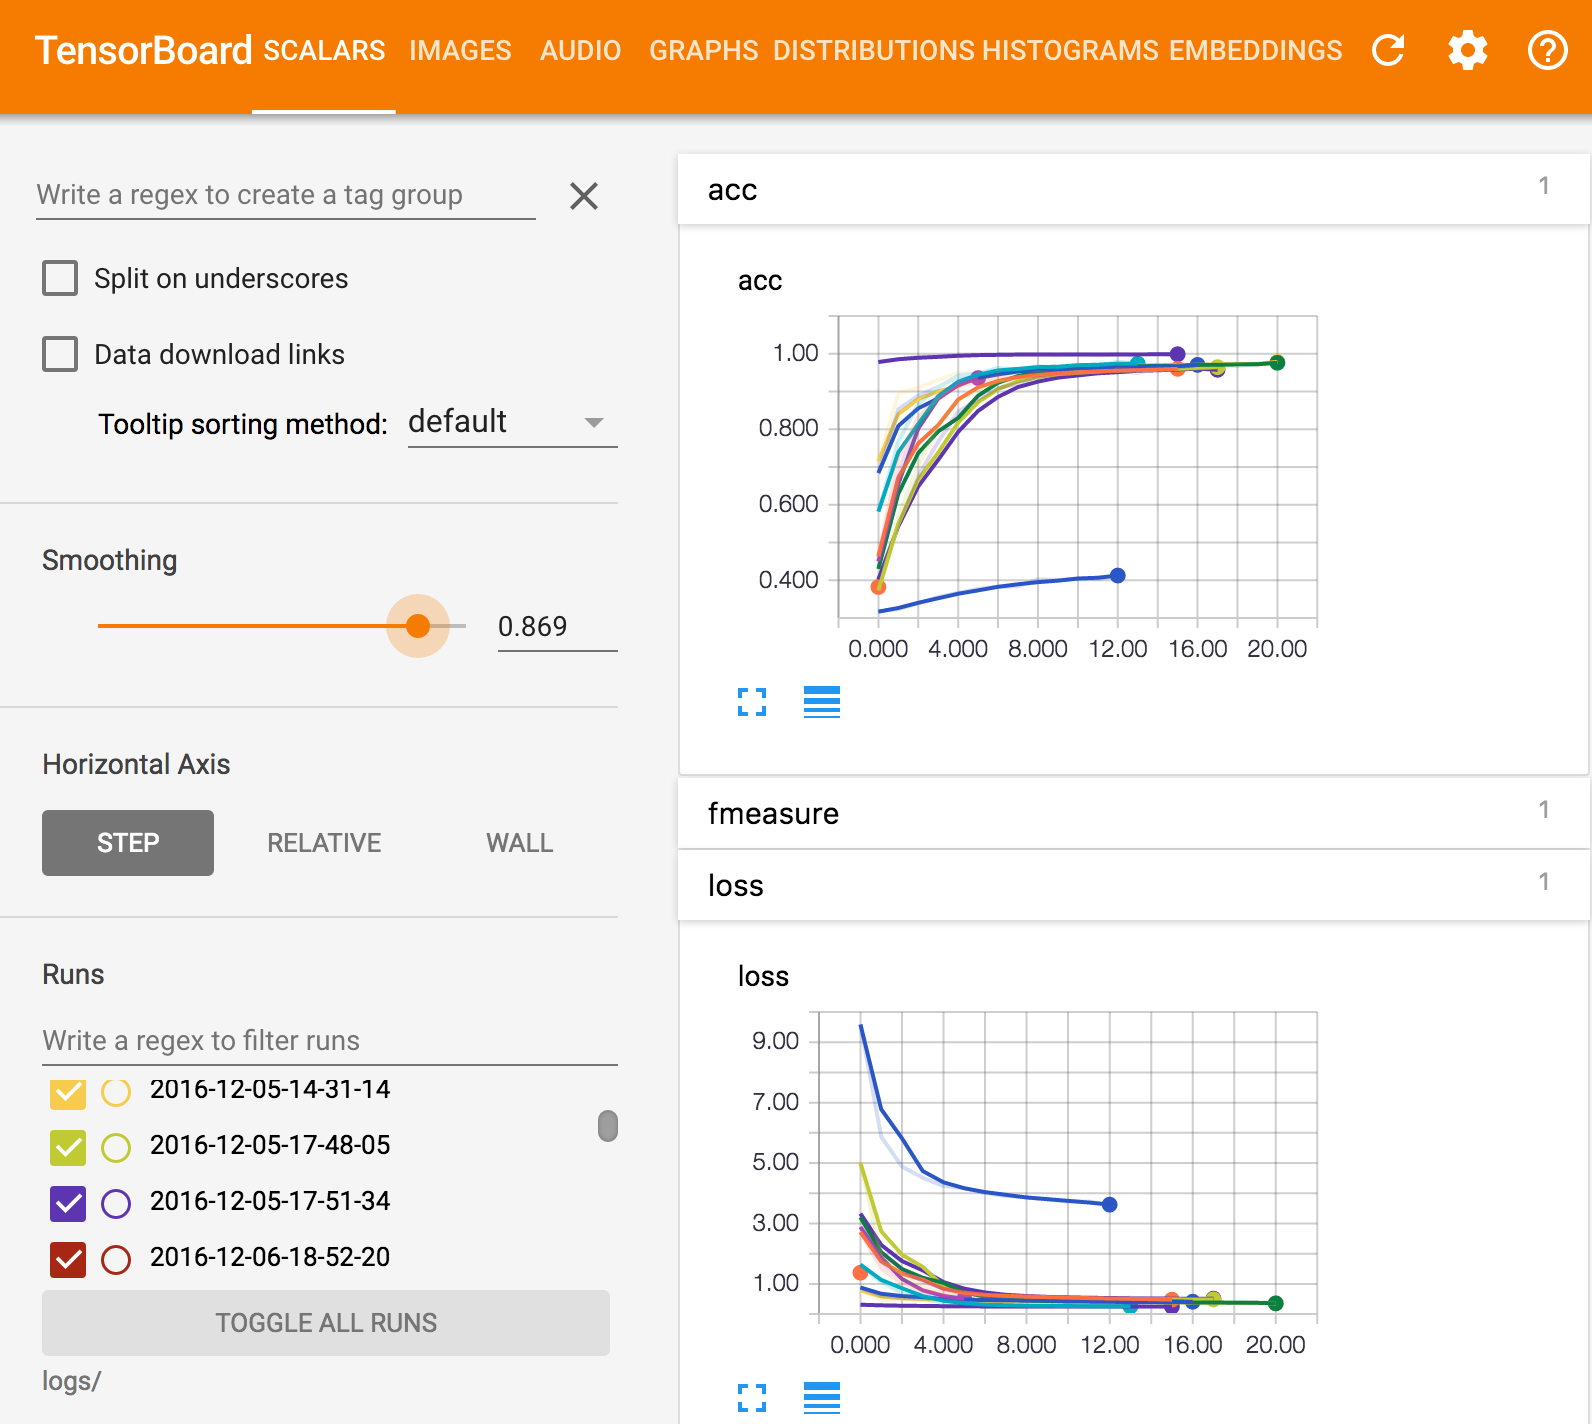
\includegraphics[width=\textwidth,keepaspectratio]{img/tensorboard.png}
    	\caption{Training accuracy and loss of different models visualized in TensorBoard. Plotting multiple evaluation measures over many training runs helped judge the overall performance progress of the system.}
    	\label{fig:tensorboard}
	\end{figure}		
	
\subsection{Data Preprocessing}
\label{sec:data_processing}
All audio files undergo preprocessing before being fed to the neural network. As a first step all files are encoded as uncompressed, lossless Waveform Audio File Format\footnote{\url{http://www.microsoft.com/whdc/device/audio/multichaud.mspx}, accessed 23.02.2017}, WAVE, commonly know by its file extension *.wav. This conversion has two advantages: A lossless data codec allows for future audio manipulations without any deterioration in signal quality and makes the data easily interchangeable for third party programs and library such as SciPy\footnote{\url{https://www.scipy.org/}, accessed 23.02.2017}. 

	Since all our neural networks do not operate on raw waveform audio signals directly we transfer our features into the image domain. As introduced in section \ref{sec:audio_representations} we used a spectrogram representation of the audio file for training our models. The spectrograms were generated using the open source command line tool SoX\footnote{\url{http://sox.sourceforge.net/}, accessed 23.02.2017}. The spectrograms are discretized using a Hann window\cite{blackman1958measurement} and 129 frequency bins along the frequency axis (y-axis) as instructed by SoX manual\footnote{\url{http://sox.sourceforge.net/sox.pdf}, page 32, accessed 26.03.2017}. Human voice frequencies for male voices begin between about 150Hz and 255Hz\cite{traunmuller1993frequency}. Female voice frequencies are usually shift by one octave and begin at 210Hz. Typically voice frequencies range up to 3.4kHz. For reference, the human ear is capable of recognizing frequencies from 20Hz to 20kHz with most sensitivity in the region of between 300Hz and 10kHz. Single sounds, however, exceed these limit significantly. Generally, voice frequencies are influenced by gender, age as well as various other factors such as the language, the type of discourse, and the emotional state of the speaker. Figure \ref{img:frequencies} shows the frequency areas with high energy in response to the tone of different vowels of human speech for the English language. Consequently, we instructed SoX to only include frequencies up to 5kHz into the spectrograms. The time axis (x-axis) is rendered at 25 pixel per second. Each audio sequence is clipped into non-overlapping ten second segments. The final segment is discarded to avoid segments shorter than the required ten seconds to avoid padding. Since we gathered enough training data we decided against padding with black pixels, which could be interpreted as silence and add unnaturally long speech pauses. We also decided against filtering silent sections within the 10 second audio segments to keep the natural pauses between words and not disturb the regular speech rhythm. Frequency intensities are mapped to an eight bit grayscale range. The resulting grayscale images are saved as lossless PNG files with 500 pixel in width and 129 pixel in height. Listing \ref{lst:spectrograms} shows the SoX command for generating a spectrogram image from an input audio file.
	
	\begin{figure}[]
  		\centering
    	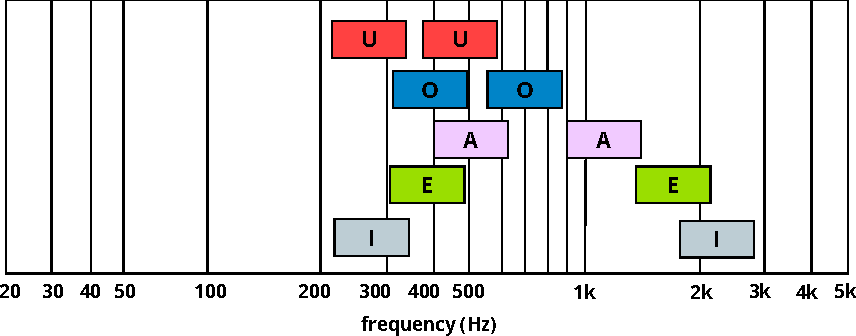
\includegraphics[width=\textwidth,keepaspectratio]{img/frequencies.pdf}
    	\caption{The upper and lower frequency areas (formant) for different vowels. These frequency ranges are typical for human speech. The lower speech formant f1 has a total range of about 300Hz to 750Hz and the higher speech formant f2 has a total range of about 900Hz up to over 3000Hz. But each single spoken tone has a much narrower range for both formants.}
    	\label{img:frequencies}
	\end{figure}	
	
	\begin{minipage}{\linewidth}
	\begin{lstlisting}[caption={SoX command and options used for generating monochrome spectrograms. All audio files were discretized into 129 frequency buckets using a constant pixel width per time step resulting into spectrogram images of 500x129 pixels.}, label={lst:spectrograms}]
    
    sox -V0 input.wav -n remix 1 rate 10k spectrogram -y 129 -X 50 -m -r -o spectrogram.png
    
    
    V0 - verbosity level 
    n - apply filter/effect
    remix - select audio channels
    rate - limit sampling rate to 10k; caps max frequency at 5kHz according to Nyquist-Shannon sampling theorem
    y - spectogram height
    X - pixels per second for width
    m - monochrome output
    r - disable legend
    o - output file
    \end{lstlisting}
    \end{minipage}
	
	As seen in figure \ref{fig:spectrogram} the spectrograms feature very apparent bright ripple-like pattern. Each of these represents a strong activation of a certain frequency at a point in time. Several frequency activations can be active simultaneously constituting a particular phoneme or sound. A sequence of these phonemes forms words and is only interrupted by short speech pauses. We hypothesize that our \ac{lid} system will learn the characteristical and unique composition of these frequency activation for every language in our classifier. 

	
	\begin{figure}[]
  		\centering
    	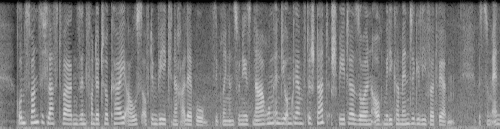
\includegraphics[width=\textwidth,keepaspectratio]{img/spectrogram.png}
    	\caption{A spectrogram generated from a ten second German audio clip  using SoX. Notice the bright ripple-like patterns representing high frequency activations. We hypothesize that these frequency activations will serve as the main features for the classifier.}
    	\label{fig:spectrogram}
	\end{figure}
	

\subsection{Neural Network Architectures}
\label{sec:cnn_architecture}
To successfully solve our research task with deep neural networks we had to design a fitting model architecture. Combing the right layers and adjusting the correct parameters is not a trivial task. Critics argue that deep learning systems are a black box and that the impact of the individual layout of the network layers is hard to understand. Therefore, we based our model architectures on proven existing designs from related work and adapted them to our needs, while heeding as best practices\cite{szegedy2016rethinking}\cite{mishkin2016systematic}.

The architecture and the number of parameters of a deep neural network suited for a given task is determined by the bias-variance tradeoff.\cite{geman1992neural} It is the goal of a network's author to avoid underfitting or overfitting on the resulting model. The bias characterizes the prediction error that results from the model's limited ability to learn relevant relations of features in the training data. Underfitting can be caused by designing too small or too few network layers causing a high bias. Variance in contrast refers to the error that results from the model responding overly sensitive to variation in the training data. By designing a too large network and Introducing too many parameters or adding too many layers results in a model with low variance. Hence, it learns an exact representation of the training data without abstracting for more general applications. This is known as overfitting.
Designing and adjusting the network layout is an iterative process. We tried many variations and parameters of our proposed model layouts to find the most suitable design for our LID system. The layout of the network interdepends and interacts with other design decisions of the system, especially the loss calculation. Each change in parameters involves a complete new training run to judge the effect of the change. Hence, the architecture always needs to be tested in its entirety. 

For this thesis we tried three different design of convolutional neural networks. The first one and second one are based on the early VGG-style CNN-M model architectures of Simonyan et al. \cite{Chatfield14}. The CNN features five convolutional layers and modest feature map output sizes. Note that the network's first two convolutional layers have comparatively large kernel size of 7x7 pixels and 5x5 pixels, respectively, yielding a large receptive field. Each convolutional layer is followed by batch normalization and a 2x2 pooling with a stride of two. We also complemented each convolutional layer with batch normalization\cite{ioffe2015batch}, a technique that helps in increasing training speed and achieving more model regularization. After the five convolutional layers we added regularization through a fifty percent dropout before flattening all parameters to a fully connected layer with 1024 outputs. The final fully connected layer serves as a classifier outputting the prediction for our language identification. Henceforth, we will refer to this model as CNN\_A. The full network layout can be seen in table \ref{tab:layers_CNN_A}.

A slightly adapted version of CNN\_A has the same amount of convolutional layers but features  a reduced number of feature maps. Instead of doubling the initial value of sixteen feature maps for every convolutional layer we stick to a schedule of 16 - 32 - 32 - 64 - 64 feature maps, respectively. The fully connected layer has also been reduceed to only 256 output units. Overall this model has significantly less parameters than the CNN\_A. The purpose of this variation is to ensure that the proposed architecture for CNN\_A is not unnecessarily complex. We called this variation CNN\_B. The full network layout can be seen in table \ref{tab:layers_CNN_A}.

	
Lastly, we evaluated architecture CNN\_C which is based on the VGG-16 network\cite{simonyan2014very} and uses constant kernel size of 3x3 for all convolutional layers. At the same time we increased the number of convolutional layers to seven and extended the number of feature map outputs for each layer: 64 - 128 - 256 -256 - 512 - 512 - 515. All fully connected layers are identical to the CNN\_A. The main difference of this network design is the smaller kernel sizes and hence a smaller receptive field of the convolutional layers. To compensate for this we increased the number of layers. The complete CNN\_C architecture is laid out in table \ref{tab:layers_CNN_C}.


For our CRNN hybrid network we constructed a convolutional neural network followed by a recurrent neural network. Specifically, we used a bidirectional long-short term memory network for the RNN part. We decided on using a bidirectional model of two LSTMs instead of a single LSTMs based on the successful results of Shi et al\cite{shi2016end}. The CNN part of the network is tasked with extracting features and providing a high dimensional intermediate frequency representation. The \ac{rnn} part interprets every vector entry along the time axis of this intermediate interpretation as a single time step.
For the CNN part we repurposed the CNN\_A network architecture of five convolutional layers with larger kernels for the first two layers. since we found this CNN layout to work best for our LID task. (Details are provided later in section \ref{sec:results_news}.) We also kept the batch normalization and max pooling layers. The bidirectional LSTM layer consist of two single LSTMs with 256 output units each. We concatenated both outputs to a vector of 512 dimensions and fed this into fully connected layer with 1024 output units serving as the classifier. The complete model architecture can be seen in table \ref{tab:layers_CRNN}. 

We decided on training both parts of the hybrid network separately. First, we trained the CNN part by itself. This simplified the task of learning frequency features for the network and saved us some time. In practical terms this meant we could reuse the model weights of the previously trained CNN\_A model. For the RNN part, we used a finetuning approach. This means we froze all convolutional layers weights by disallowing any further weight updates during the tracing phase. The bidirectional LSTM and \ac{fc} layers, however, remained unfrozen and continued to be subject to weight updates and hence was trained regularly.

 \begin{table}[]
  \centering
  \begin{tabularx}{\textwidth}{Xcccc}
  \toprule
Layer Type                    & \multicolumn{2}{c}{output size} & kernel & stride  \\ 
                                                    & CNN\_A & CNN\_B &      &     \\\midrule

\mbox{Convolution with} \mbox{Batch Normalization}  & 16     & 16   & 7x7    & 1   \\ 
Max Pooling                                         & 16     & 16   & 2x2    & 2   \\ 
\mbox{Convolution with} \mbox{Batch Normalization}  & 32     & 32   & 5x5    & 1   \\ 
Max Pooling                                         & 32     & 32   & 2x2    & 2   \\ 
\mbox{Convolution with} \mbox{Batch Normalization}  & 64     & 32   & 3x3    & 1   \\ 
Max Pooling                                         & 64     & 32   & 2x2    & 2   \\ 
\mbox{Convolution with} \mbox{Batch Normalization}  & 128    & 64   & 3x3    & 1   \\ 
Max Pooling                                         & 128    & 64   & 2x2    & 2   \\ 
\mbox{Convolution with} \mbox{Batch Normalization}  & 256    & 64   & 3x3    & 1   \\ 
Max Pooling                                         & 256    & 64   & 2x2    & 2   \\ 
Dropout \& Flatten                                  & 3328   & ??   &        &     \\ 
\mbox{Fully Connected}                              & 1024   & 256  &        &     \\ 
\mbox{Fully Connected}                              & 4      & 4    &        &     \\ 
  \bottomrule
  \end{tabularx}
  \caption{The layerwise architecture for the convolutional neural network CNN\_A and CNN\_B. This design is based on the early VGG style networks and features large kernel size for the first two convolutional layers in an effort to capture a large receptive field of features.}
  \label{tab:layers_CNN_A}
  \end{table}


  \begin{table}[]
  \centering
  \begin{tabularx}{\textwidth}{Xccc}
  \toprule
Layer Type                                          & output size  & kernel & stride \\ \midrule
\mbox{Convolution with} \mbox{Batch Normalization}  & 64     & 3x3    & 1x1  \\ 
Max Pooling                                         & 64     & 2x2    & 2x2  \\ 
\mbox{Convolution with} \mbox{Batch Normalization}  & 128    & 3x3    & 1x1  \\ 
Max Pooling                                         & 128    & 2x2    & 2x2  \\ 
\mbox{Convolution with} \mbox{Batch Normalization}  & 256    & 3x3    & 1x1  \\ 
\mbox{Convolution with} \mbox{Batch Normalization}  & 256    & 3x3    & 1x1  \\ 
Max Pooling                                         & 256    & 2x2    & 2x2  \\ 
\mbox{Convolution with} \mbox{Batch Normalization}  & 512    & 3x3    & 1x1  \\ 
\mbox{Convolution with} \mbox{Batch Normalization}  & 512    & 3x3    & 1x1  \\ 
Max Pooling                                         & 512    & 2x2    & 2x2  \\ 
\mbox{Convolution with} \mbox{Batch Normalization}  & 512    & 3x3    & 1x1  \\ 
Max Pooling                                         & 512    & 2x2    & 2x2  \\ 
Flatten                                             & 6144   &        &      \\                        
\mbox{Fully Connected}                              & 1024   &        &      \\
\mbox{Fully Connected}                              & 4      &        &      \\
  \bottomrule
  \end{tabularx}
  \caption{The layerwise architecture for the convolutional neural network CNN\_C. With seven convolutional layers this network design is deeper than the other two proposed CNN architectures. Additionally, the number of feature maps were increased to 512 units compared to the 256 units of the CNN\_A network. Overall this network is deeper and consists of a high number of parameters than the other two designs.}
  \label{tab:layers_CNN_C}
  \end{table} 
    
    
  \begin{table}[]
  \centering
  \begin{tabularx}{\textwidth}{Xccc}
  \toprule
Layer Type                                          & output size    & kernel & stride  \\ \midrule
\mbox{Convolution with} \mbox{Batch Normalization}  & 123 x 494 x 16  & 7x7    & 1x1     \\ 
Max Pooling                                         & 61 x 247 x 16   & 2x2    & 2x2     \\ 
\mbox{Convolution with} \mbox{Batch Normalization}  & 57 x 243 x 32   & 5x5    & 1x1     \\ 
Max Pooling                                         & 28 x 121 x 32   & 2x2    & 2x2     \\ 
\mbox{Convolution with} \mbox{Batch Normalization}  & 26 x 119 x 64   & 3x3    & 1x1     \\ 
Max Pooling                                         & 13 x 59 x 64    & 2x2    & 2x2     \\ 
\mbox{Convolution with} \mbox{Batch Normalization}  & 11 x 57 x 128   & 3x3    & 1x1     \\ 
Max Pooling                                         & 5 x 56 x 128    & 2x2    & 2x1     \\ 
\mbox{Convolution with} \mbox{Batch Normalization}  & 3 x 54 x 256    & 3x3    & 1x1     \\ 
Max Pooling                                         & 1 x 53 x 256    & 2x2    & 2x1     \\ 
Permute                                             & 53 x 1 x 256    &        &         \\
Reshape                                             & 53 x 256        &        &         \\
\mbox{Bidirectional LSTM}                           & 1024            &        &         \\
\mbox{Fully Connected}                              & 4               &        &         \\
  \bottomrule
  \end{tabularx}
  \caption{The layerwise architecture for the convolutional recurrent neural network.}
  \label{tab:layers_CRNN}
  \end{table}
  
  
  \todo{why not automatic design?}
  \todo{why not rectengular kernels?}
